% !TEX root = thesis.tex
\startchapter{Methodology and Constructs}
\label{chap:meth}
Before we dive into our actual studies of the effect of socio-technical congruence and its use to form recommendations, we present the overall roadmap for this thesis (Section~\ref{c5:sec:roadmap}) and some common definitions (Section~\ref{c5:sec:definitions}) and constructs (Section~\ref{c5:sec:constructs}) that we use for the remainder of the thesis.
Furthermore, we also will discuss the general approach to the data collection methods employed (Section~\ref{c5:sec:datacollection}).

\begin{figure}[h!]
\centering
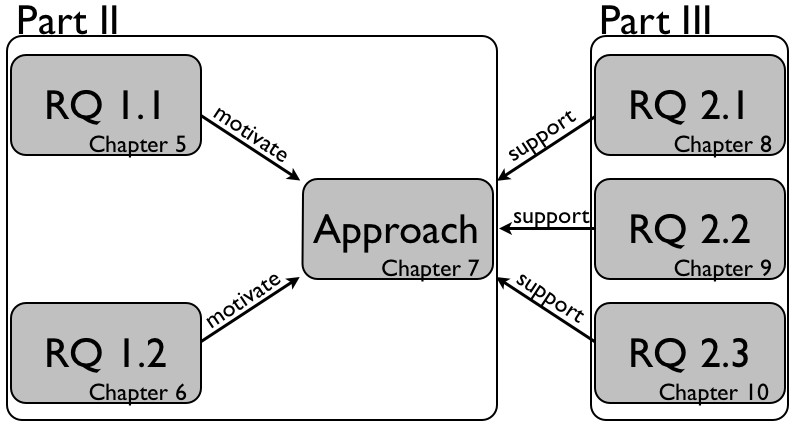
\includegraphics[height=.9\textheight]{./figures/roadmap}
\caption{What chapter addresses which research questions in relation to our approach to improve social interactions among software developers.}
\label{fig:roadmap}
\end{figure}

\section{Methodology Roadmap}
\label{c5:sec:roadmap}
In this section we discuss the methods we apply to answer the research questions presented in Chapter~\ref{chap:bg}.
Figure~\ref{fig:roadmap} depicts the relationship between the research questions and the contribution of this thesis, an approach to improve social interactions among developers by characterizing the quality of interactions by the build outcome of the related build.
Research questions~1.1 and~1.2 discussed in Chapters~\ref{chap:soc-net} and~\ref{chap:stc-net2} motivate the approach.
Research questions~2.1 and~2.3 (Chapters~\ref{chap:stc-net} and~\ref{chap:actionable}) explore whether socio-technical networks can be used to form recommendations that can prevent build failures, whereas research question~2.2 inquires in Chapter~\ref{chap:talk} whether such recommendations are acceptable by developers.

\subsection{Research Question 1.1}
%Motivation
\begin{description}
  \item[RQ 1.1:] Do Social Networks influence build success? (Chapter~\ref{chap:soc-net})
\end{description}
The thesis goal is to design an approach that is able to improve the social interactions in the form of communication among software developers.
As a first step we need to establish if the communication among software developers has an influence on the build success.

%Data Source
We have access to the development repositories used by the IBM Rational Team Concert development team such as their source code management system, communication repositories in the form of work item discussions, and their build results.
All these artifacts are linked together in a way that we can trace from the build result which changes went into the build and which work items a change is meant to implement.

%Methods
Using this information we can construct social networks from all the work items that are related to builds.
These networks are then described using social network metric and form the input for machine learning algorithms to predict whether a build based on these metrics is more likely to fail or succeed.

%Expected results
Via this machine learning approach we want to establish a connection between a build's social network and its outcome. 
If we are able to predict the build outcome more accurately than by simply guessing, using the likelihood for a build failure, we demonstrated that there is a statistical relationship between build outcome and social networks.
Thus, this result forms the first evidence that manipulating the social network might yield a positive effect on build success.

\subsection{Research Question 1.2}
\begin{description}
  \item[RQ 1.2:] Does Socio-Technical Networks influence build success? (Chapter~\ref{chap:stc-net2})
\end{description}

%Motivation
Knowing that a social network can influence the success of the corresponding build leads us to the question of how networks should be manipulated to improve the likelihood for a build to succeed.
Therefore, we explore the relationship between socio-technical networks generally and gaps within that networks, with a gap being formed by two developers that share a technical dependencies but did not communicate about work related to the build of interest, and build success.
%Data Source
Similarly to the previous research question, we base the analysis on the same data set, as it allows us to directly infer technical relationships among developers related to a software build from the changes submitted to the source code management tool.
We used these changes previously to infer the work items developers used to communicate among each other about the build.

%Methods
Since the socio-technical networks has two semantically different edges connecting two developer within a network (technical dependencies and communication among developers) we refrain from using social network metrics as they assume only one mode of connection among nodes within a network.
Instead we investigate the relationship of the socio-technical congruence index and build success as well as focusing on the influence of gaps in the network on build success.

%Expected results
Via statistical analysis methods such as regression analysis we want to establish a relationship between the existence of gaps within the socio-technical network and build success.
By addressing this research question we obtain another piece of evidence that let us formulate an approach to recommend actions to increase build success that are specifically alleviating gaps within the socio-technical network by recommending developer to communicate.

\subsection{Research Question 2.1}
\begin{description}
  \item[RQ 2.1:] Can Socio-Technical Networks be manipulated to increase build success? (Chapter~\ref{chap:stc-net})
\end{description}
%Motivation
The previous two research questions enable us to formulate an approach to generate recommendations that are meant to foster communication among developers in order to increase build success.
This leads to the next step, namely, to explore whether this approach can generate recommendations that bear a statistical relationship to build success.

%Data Source
With the same data source we used to explore the previous two research questions, we try to relate individual reoccurring gaps in socio-technical networks to build failure.
%Methods
Knowing those gaps, or developers that frequently share a technical dependency without communicating with respect to a build that failed we check if adding a social dependency would change the likelihood of a build to fail.
%Expected results
We expect to find a number of gaps that when mitigated increase the likelihood of build success.

\subsection{Research Question 2.2}
\begin{description}
  \item[RQ 2.2:] Do developers accept recommendations based on software changes to increase build success? (Chapter~\ref{chap:talk})
\end{description}
%Motivation
Before exploring if the recommendation hold actual value with preventing build failures, we explore if developers would welcome recommendations with respect to changes.
%Data Source
Therefore, we joined the development effort of one of the Rational Team Concert development teams as participant observer to get an insight into how the actual developer communicate during their day to day work.

%Methods
We complement these observations with followup interviews to gain a better understanding of the team dynamics and their discussion topics, since as a project newcomer our work is limited to more basic tasks in contrast to higher level decision making.
To extend our reach beyond the local team we deployed a questionnaire with the product team at large to gain a better understanding whether the recommendations we would supply can easily be integrated in their typical discussions with fellow developers.

%Expected results
This study should give us a better understanding of whether developers are discussing individual changes, thus justifying the appropriateness of the level of recommendations.
Furthermore, we expect to uncover general suggestions on when and how to supply such recommendations as developers might not always be interested in individual changes even if they pose a threat to build success.

\subsection{Research Question 2.3}
\begin{description}
  \item[RQ 2.3:] Can recommendations actually prevent build failures? (Chapter~\ref{chap:actionable})
\end{description}
%Motivation
We conclude our evaluation of our proposed approach with  a proof of concept in a more controlled environment to ascertain whether the recommendation we can generate actually help in preventing builds from failing.
As root cause analysis of failures can be very tedious and due to the various reasons a build can fail that are not necessarily due to software changes we depart from studying the development of Rational Team Concert and observe students extending an open source project during a course taught at the University of Victoria, Canada, and Aalto University, Finland.

%Data Source
This different setting allows us to ask the study participants to use tools we developed to collect more fine grained data on their development efforts, such as when they edited which parts of the source code.
Additionally, we have access to the actual source code repositories such as source code management, issue tracking, email, and text chat sessions.
Furthermore, we ask the students to answer regular questionnaires and keep a development diary that are meant to collect information on issues that the students encounter during the course and are especially related to their development effort.

%Methods
Analyzing the collected data from the questionnaires and development diaries is done manually, by reading and annotating the different responses and entries to uncover build issues that were important to the students.
Knowing the build issues the students encountered, we select the most severe in terms on the number of reports and trace them to the actually root cause if possible by identifying the code changes that causes them (if applicable) and continuing to analyze the offending changes and identifying corresponding communication.

%Expected results
We expect to find one representative example of a failed build that the students encounter during the course that can be resolved using recommendations based on information that is available before the students actually incorporate their modifications in to the source code repository of the project.

\section{Definitions}
\label{c5:sec:definitions}
We start with defining three constructs that we are heavily relying upon: (1) Work Item being a complete unit of work, (2) Change-set being the technical work submitted by a developer, and (3) builds referring to a testable product.

\subsection{Work Item}
A \emph{Work Item} is a unit of work that can be assigned to a single developer.
A unit of work can span anything from being a bug-report, reported by either the end user or by a developer, to a feature implementation.
\emph{Work Item}s can be hierarchically organized to show the work break-down from high-level requests to manageable pieces.
One project team member is responsible for a work item to be completed, the sub work items that it is broken-down to do not necessarily need to be assigned to the owner of the parent work item.

For instance, in the case of the IBM Rational Team Concert the development team creates story items to describe larger functionality from the user point of view and assigns them depending on the complexity and implication of the story.
The owner of the story then either breaks down the story into multiple stories or tasks which are again assigned to team members according to their complexity and implications.
Once the work item level is sufficiently low the developer assigned to it can make the necessary modifications to the project to accomplish the work detailed in the work item.

\begin{note}
\begin{mydef}
A \emph{Work Item} is a defined and assignable unit of work.
\end{mydef}
\end{note} 

\subsection{Change-Set}
A \emph{Change-Set} is a set of source code changes applied to a number of source code files, with a file being the artifact that a developer would change to add to, modify, or delete from the current product. 
The developer that applied those changes to the product bundles them into one or multiple change-sets.
For example, in the Eclipse project\footnote{\url{http://www.eclipse.org}} the developers use CVS\footnote{\url{http://www.nongnu.org/cvs}} as their version control system to manage changes to the Eclipse IDE.
A developer will check out her current version of the repository and started editing, creating and deleting files in order to fulfill a work item she is currently working on.
Once the developer decides that she accomplished the work to finish her current work item, she commits her changes.
Those changes that consists of file creations, deletions, and modifications taken together are referred to as a \emph{Change-Set}. 

\begin{note}
\begin{mydef}
A \emph{Change-Set} is a set of modifications, additions, and deletions of software artifacts such as source code files, classes or methods.
\end{mydef}
\end{note}

\subsection{Build}
The goal of each software development team is to deliver a finished or improved product at some point in time.
This finished product is often referred to as the final \emph{Build}.
A \emph{Build} can generally be referred to as any instance of the product that can be run to some extend.
To create a build a team gathers all the changes implementing work items that are required for the new build and compiles and packages the product.
The amount of work items and their respective changes included in a build will gradually increase over time because more work will be finished as the project progresses.

In the case of the IBM Rational Team Concert development team, they create builds on a frequent basis to test the product as a whole to look for integration issues. 
The team also subscribes to the philosophy to use their own products themselves and thus try to bring each build to a level that it can be used for development.
This intense use enables the team to spot issues that are still within the product and enables them to asses the severity of those found issues.

\begin{note}
\begin{mydef}
A \emph{Build} is a to some extend executable version of the product that includes a number of changes implementing work items.
\end{mydef}
\end{note}

\section{Constructs}
\label{c5:sec:constructs}
From the definitions introduced previously we can derive the three central constructs we work with in this thesis: (1) the social network connecting communicating and coordinating developers, (2) the technical network connecting developer that are dependent through code artifacts, and (3) the socio-technical network that combines the social and technical network in a meaningful way.
These constructs are important for the three chapters that are mining the repository provided by the Rational Team Concert development team (Chapters~\ref{chap:soc-net},~\ref{chap:stc-net2}, and~\ref{chap:stc-net}).

\subsection{Social Network}
\begin{figure}[t!]
\begin{center}
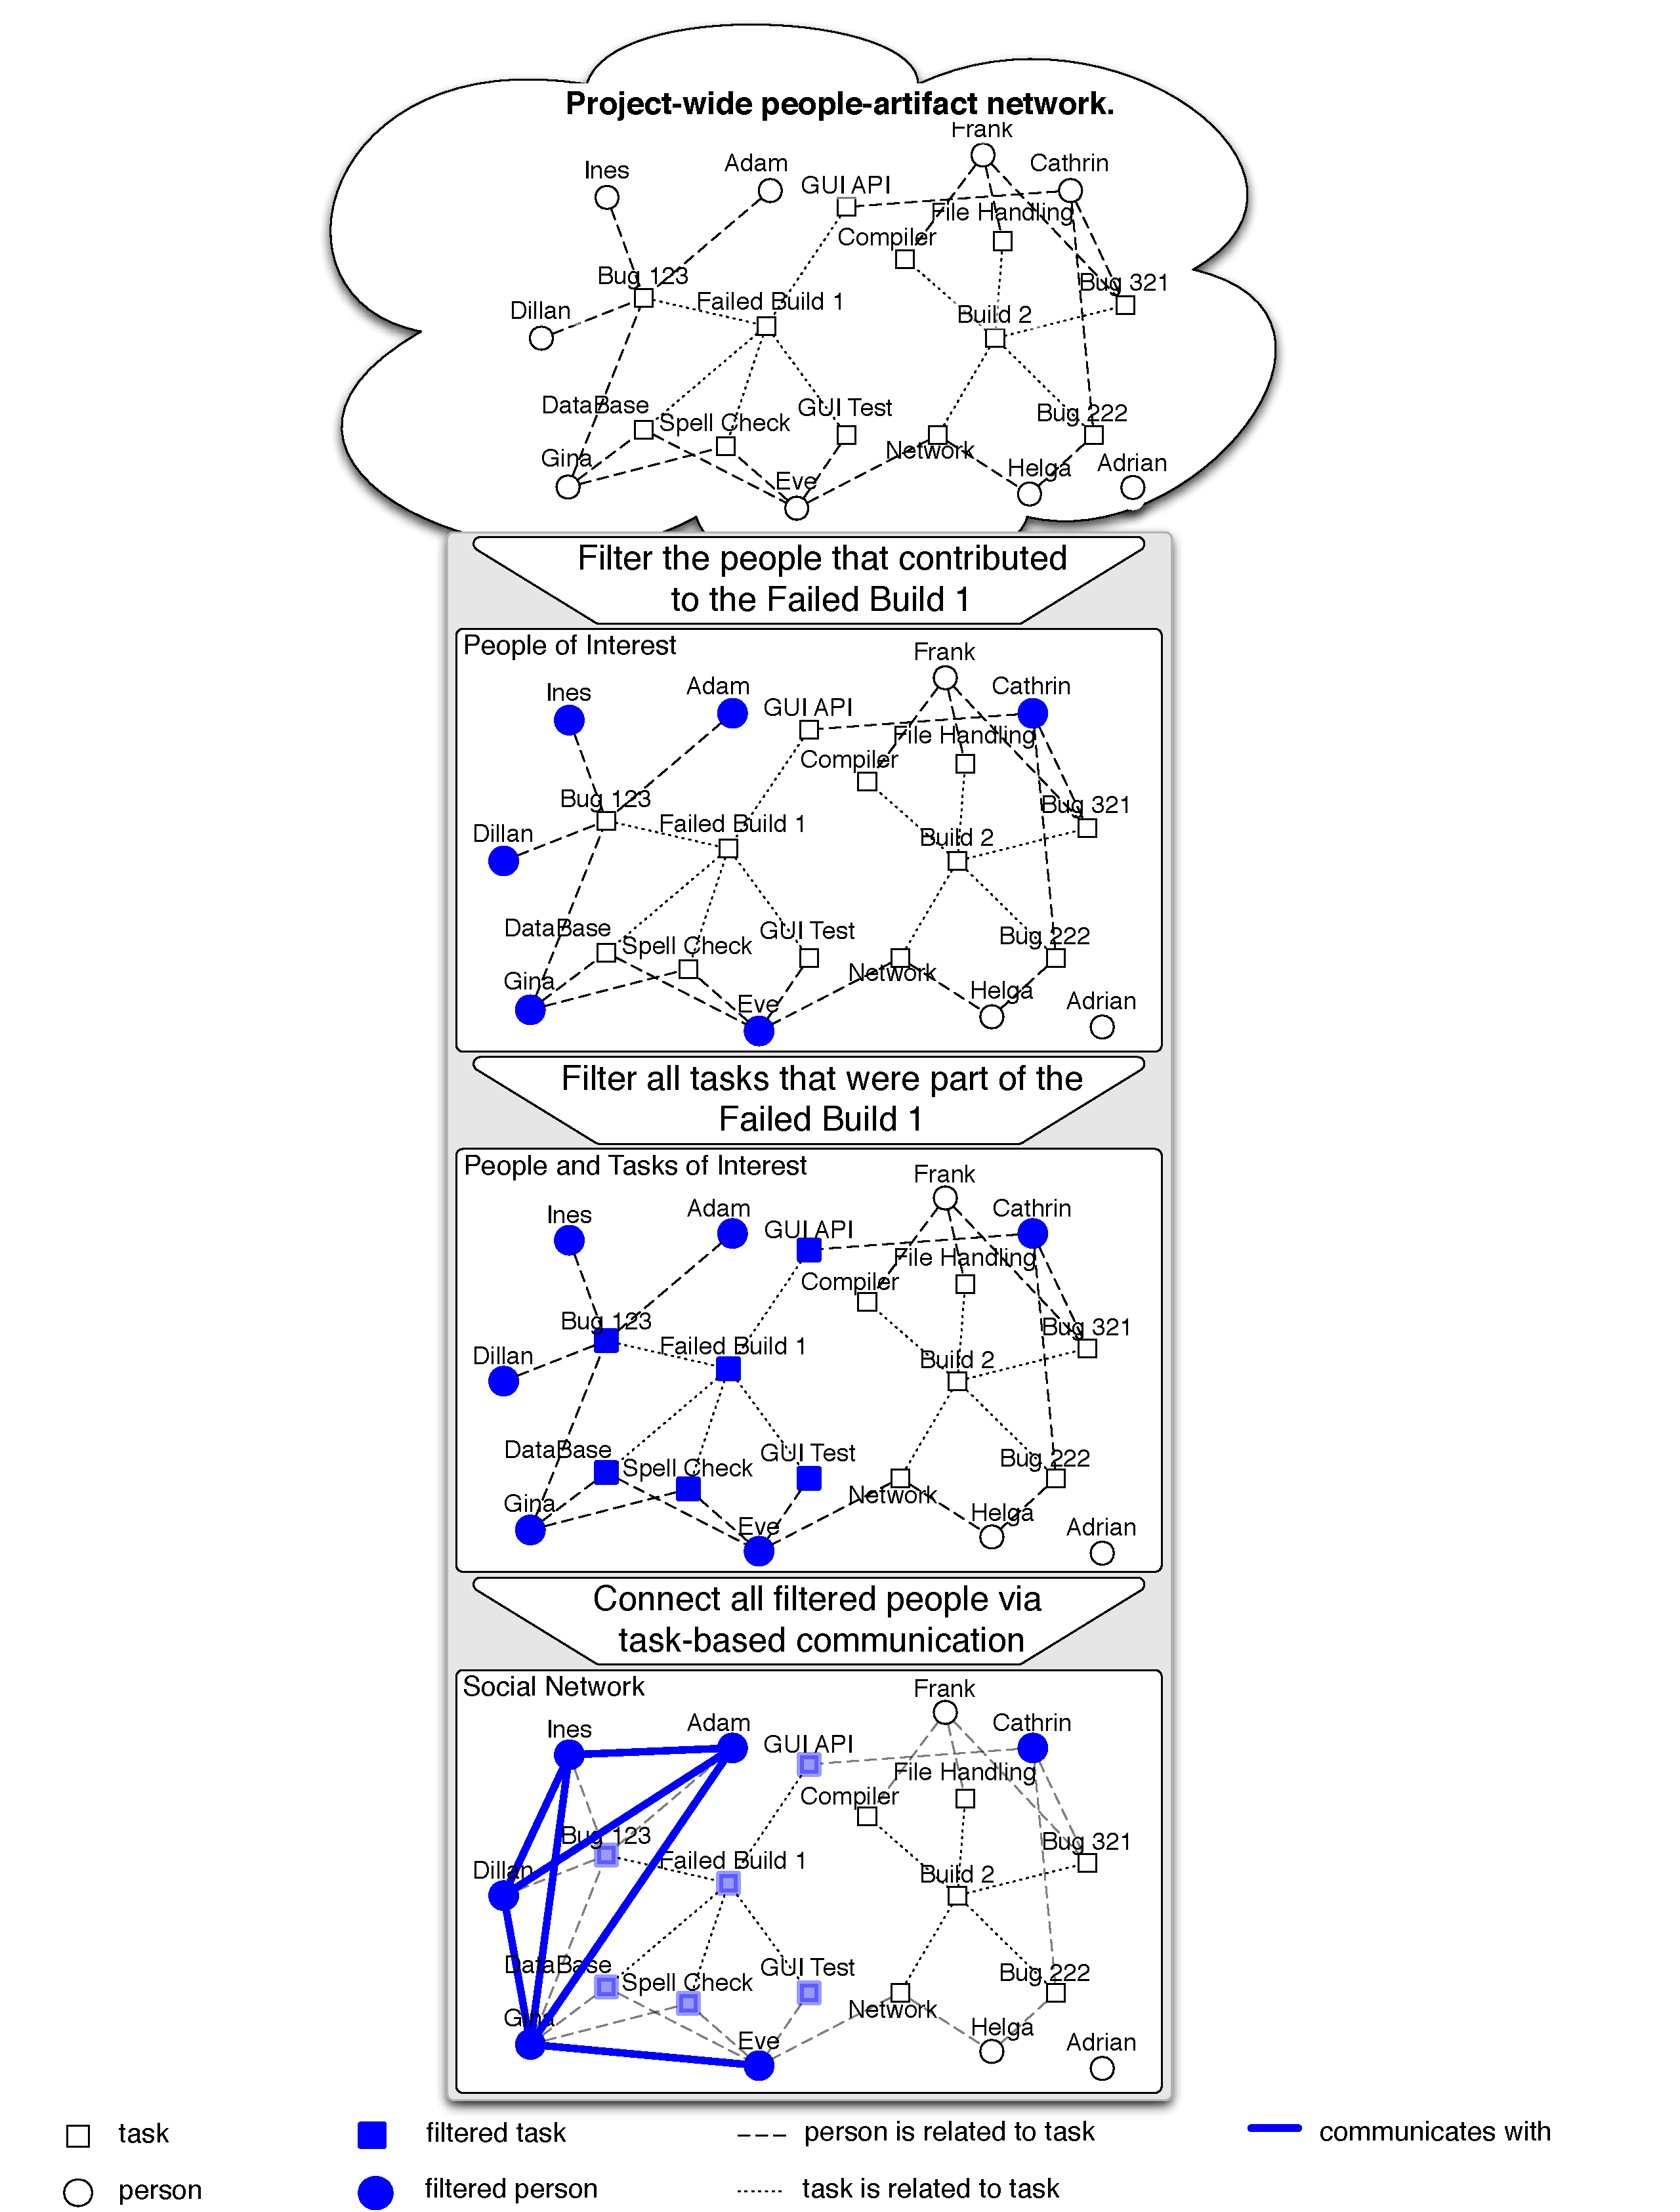
\includegraphics[height=1.3\textwidth]{./figures/grand_figure}
\caption{Social network construction examples in our approach}
\label{fig:network}
\end{center}
\end{figure}
To illustrate our approach to construct social networks we go through the example of a failed build illustrated in Figure~\ref{fig:network}. 
A social network is represented as a graph that consist of nodes connected by edges. 
In our approach, the nodes represent people and edges represent task-related communication between these people.

The approach is repository and tool independent and can be applied to any repositories that provide information about people, tasks, technical artifacts, and communication, this includes work, issue, or change management repositories, such as Bugzilla or IBM Rational Team Concert; or source code management systems, such as CVS or IBM Rational Team Concert; or even communication repositories such as email archives.

We construct and analyze social networks within a collaboration scope of interest.
With a collaboration scope defining the people and interactions of interest.
In this example, around Failed Build 1, the collaboration scope is the communication of the contributors to the failed build. 
Other examples include the collaboration of people working on a critical task, in a particular geographical location, or in a functional team such as testing.

There are three critical elements that are necessary to construct task-based social networks for a collaboration scope and that need to be mined from software development repositories:

\begin{description}
\item[Project Members] are people who work on the software project. 
These project members can be developers, testers, project managers, requirements analysts,
or clients. 
Project members, such as Cathrin and Eve, become nodes in the social network.

\item[Work Items] are units of work (as defined earlier) within the project that may create a need to collaborate and communicate. 
Examples for a work item include resolving Bug~123 or implementing the GUI API. 
More generally, implementing feature requests and requirements can also be considered collaborative tasks.

\item[Work Item Communication] is the information exchanged while completing a work item and is the unique information that allows us to build task-based social networks. 
In our example, dashed black lines represent task-related communication such as a comment on Bug 123, or an email or chat message about GUI API.
Task-related communication is used to create the edges between developers in the social networks.
\end{description}

The data underlying the social network used throughout this thesis are based on work items and their associated discussions.
In IBM Rational Team Concert each work item has an attached discussion thread were developers can discuss the work item or simply note down their thoughts while working on the work item.
This means, we would create a link between two developer if they comment together on the same work item to indicate that they are part of the same discussion.
Note that this sections draws heavily from our work done in collaboration with Timo Wolf, Daniela Damian, Lucas Panjer, and Thanh Nguyen~\cite{wolf:ieee:2009}.

\subsection{Technical Network}
\begin{figure*}[t!]
\centering
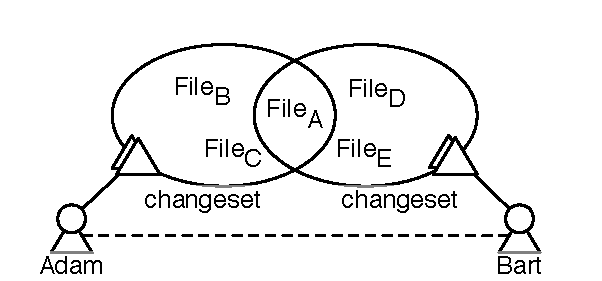
\includegraphics[width=.7\textwidth]{figures/cochangedfiles}
\caption{Creating a technical network by connecting two developer that changed the same file.}
\label{fig:addtechnicaledge}
\end{figure*}

% some preamble as in the previous subsection
Building technical networks follows a very similar approach as we described for building social networks.
In fact, the technical network is a social network whose main distinction from the social network described earlier lies in the way edges between nodes are created.
We derive the name of technical network from the way we link developer with each other, namely if they are modifying related source code artifacts.
As in the previous network construction, the construction of the technical network is based on three components:

\begin{description}
\item[Project Members] are people who work on the software project. 
These project members can be developers, testers, project managers, requirements analysts,
or clients or in general anyone that modifies software artifacts through change-sets. 
In Figure~\ref{fig:addtechnicaledge} project members, such as Alfred and Bob, become nodes in the technical network because they modified the same file.

\item[Change-Sets] are changes made to software artifacts by individual users. 
A set consists of a number of artifacts that have been modified as well as the modifications themselves.
For example Alfred as shown in Figure~\ref{fig:addtechnicaledge} modified File$_{\text{A}}$ and File$_{\text{B}}$.

\item[Software Artifact Relation] describe the relation between developers in the technical networks.
These relationship can be defined in several different ways.
For example, in Figure~\ref{fig:addtechnicaledge} Alfred and Bob are related through a technical relationship because they modified the same file.
Note, that we are mostly interested in relationships between artifacts that are effected by changes.
\end{description}

% Example as shown in the picture
Constructing technical networks therefore follows three steps: (1) we gather all the change-sets of interest, (2) identify the relations between artifacts, (3) infer from the change-sets and the relations between the source code artifacts the relation between the artifact owners.
For example, after we selected the set of change-sets of interest we define the change-sets themselves as the source code artifact and identify the owners of those artifacts.
Then we infer the relationship between those source code artifacts by relating all change-sets that changes the same source code file.
And as Figure~\ref{fig:addtechnicaledge} shows this means in the case for Alfred and Bob that they are connected because both own a change-set that modifies the same file.

\subsection{Socio-Technical Network}
\begin{figure}[t!]
%	
  \centering
  \subfloat[Inferring to the build focus relevant change-sets and work items.]{
    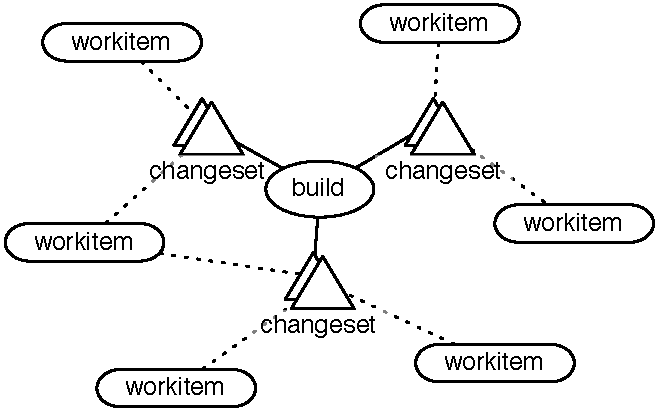
\includegraphics[width=.46\textwidth]{figures/buildworkitem}
    \label{fig:construct-focus}
  }
 % 
  \hspace{8pt}
  \subfloat[Constructing an social networks from work item communication.]{
	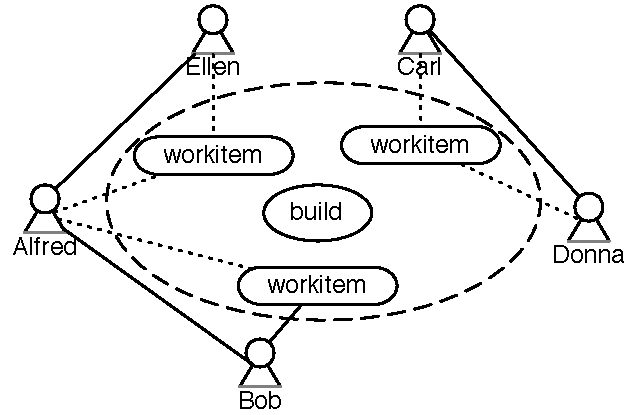
\includegraphics[width=.46\textwidth]{figures/buildsn}
     \label{fig:construct-sn}
  }
  
    \subfloat[Linking developers in a technical networks via change-set overlaps.]{
  	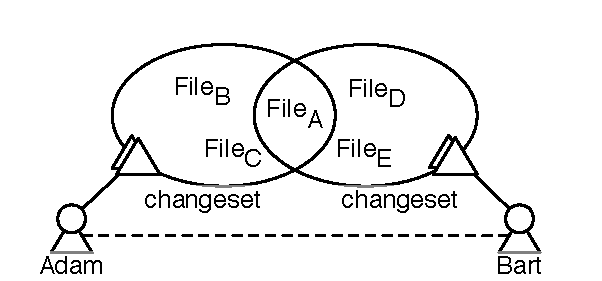
\includegraphics[width=.46\textwidth]{figures/cochangedfiles}
    \label{fig:construct-tn}
  }
  %
    \hspace{8pt}
  \subfloat[Combine social and technical networks into a socio-technical network.]{
  	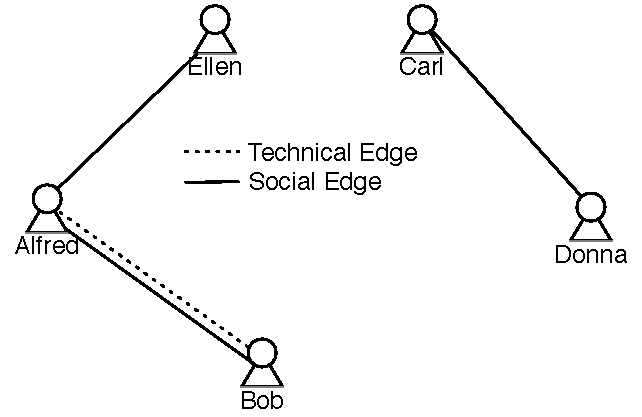
\includegraphics[width=.46\textwidth]{figures/stc-net}
	\label{fig:construct-combine}
  }
  \caption{Constructing socio-technical networks from IBM Rational Team Concert data.}
  \label{fig:construct-stc}
\end{figure}

Socio-Technical networks are a meaningful combination of both social and technical networks.
Selecting this meaningful combination reflects itself in the selection of the work-items in the case of building the social network and selecting the change-sets and their relations in the case of the technical network.
Hence constructing a socio-technical network requires the following four steps:

\begin{enumerate}
\item\textbf{Selecting the Focus} used for the socio-technical network represents the glue that binds the social and technical network into a socio-techncial network. 
This focus also referred to as filter in our earlier publication~\cite{wolf:ieee:2009}, determines the content of the networks.
In this thesis we use for the focus of such networks are software builds to construct networks that are describing the coordination among developer for a given software build.
\item\textbf{Constructing the Social Network} follows the description above with the focus determining the work items that are selected to generate the nodes from the work item participants and the edges from the communication among the participants through a work item.
\item\textbf{Constructing the Technical Network} follows the description of constructing technical networks above with the focus determining the change-sets being used to determine and connect developers in the network.
\item\textbf{Combining Networks} is the final step that overlays the networks by unifying the set of developers in both networks.
Thus a pair of developers can be directly connected with each other through two edges, one representing the edge from the technical network and the other the edge from the social network.
\end{enumerate}

% describe the example in the figure
Figure~\ref{fig:construct-stc} shows an example on how we in our studies of the IBM Rational Team Concert development team used to create socio-technical networks.
In the first step (Figure~\ref{fig:construct-focus}) we set the focus to be a software build which allows us via the change-sets that made it into the build to infer what work items are also represented in said build.
Given the focus, the social network can be constructed using the work items that can be linked to the software build (Figure~\ref{fig:construct-sn}).
Similarly the construction of the technical network relies on the change-sets that went into a build. 
To actually infer edges between developer, we relying on co-changed files within a build as an indicator of work dependency (Figure~\ref{fig:construct-tn}).
Finally, the two networks are combined and yield the socio-technical network shown in Figure~\ref{fig:construct-combine}.

\section{Data Collection Methods}
\label{c5:sec:datacollection}
To conduct the research for this thesis we drew upon multiple data sources.
We employ repository mining techniques to identify larger trends in measurable activities.
In contrast to gain a more in-depth understanding on how developers actually work and deal with interdependencies especially how they would react to certain recommendations and whether they are can be made useful we employ qualitative methods.

\subsection{Repository Mining}
Software development usually uses a number of tools to manage information electronically such as version archives and issue trackers.
Additionally to storing source code and tasks/issues, those software repositories can also contain digital communication such as forum and email discussions or logs of IRC\footnote{\url{http://en.wikipedia.org/wiki/Internet_Relay_Chat} last visited June 8th, 2012} or instant messenger chats.

Repositories can grow to considerable sizes depending on the projects live span and intensity. 
Therefore, it is often infeasible to manually review the history of a project and it is necessary to employ data-mining techniques to be able to analyze trends.
Although this approach is limited in gaining a deeper understanding of the intricacies of a development project, it nevertheless is invaluable to place in-depth results in the bigger picture of the project.
Furthermore, data mining approaches are one way to easily give back value to the development team without burdening any individual developer with diverting time to other non-automatic data collection instruments.
This is an important point as one goal of this thesis is to explore the ability of the concept of socio-technical congruence to generate actionable recommendations.
In case a developer needs to personally provide a large amount of information manually the overhead generated by a system might outweigh the benefit of recommendations and therefore make the system useless.

We extract information from three different types of repositories: (1) version control, (2) task management, and (3) build engine systems.
The version control supplies us with the knowledge on how developers are connected through their technical work.
The task management supplies us with the information on who communicated with whom with respect to a work item.
And lastly the build engine supplies us with the focus to construct socio-technical networks.

In order to derive socio-technical networks we need to link the different artifact types.
Within IBM Rational Team Concert as illustrated in Figure~\ref{fig:construct-focus} work items are linked to change-sets and change-sets are linked to builds, therefore, establishing the connections needed to construct socio-technical networks with a build as focus.
Similarly these links can be inferred as proposed by Cubranic et al~\cite{cubranic:tse:2005} from repositories that are missing the capabilities of creating formalized links.
We used repository mining techniques in Chapter~\ref{chap:soc-net},~\ref{chap:stc-net2}, and~\ref{chap:stc-net} to explore the rich repositories provided by the IBM Rational Team Concert team.

\subsection{Surveys}
To complement the insights we obtained from mining repositories we use surveys.
Surveys are designed iteratively and piloted before deployment, and intended to collect input to enrich and clarify information obtained from the software repositories. 
With each survey we try to minimize the time each developer needs to spend completing them, which usually limits ourselves to focus on closed questions offering prepared answers.
We constrain ourselves in this way to minimize the distraction to each individual developer and thus increase the response rate.

Our surveys are deployed through web services to make the collections more convenient to each developer as they are spending most of their times working at a computer enabling them to fill out the survey at their earliest convenience.
Keeping track of a paper version is more cumbersome as they might not easily be returned, especially considering that the development teams we are collaborating with are distributed across different continents.

We both deployed surveys working with the Rational Team Concert development team (Chapter~\ref{chap:talk}) and when working with students working on a large course project at the University of Victoria, Canada, and Aalto University, Finland (Chapter~\ref{chap:actionable}).


\subsection{Observations}
The next richer and also to the developer more distracting method of data gathering are observations.
Although not necessarily actively interrupting and distracting developer, the act of observing can distract developers and also change their behaviour.
In order to minimize this type of distraction and to mitigate the observer bias, we employed a special form of observation study namely participant observation.
In short we became both an observer and a participant.
%
Being a participant observer has a multitude of advantages:

\begin{itemize}
\item\textbf{Reciprocity.} By participating in the actual development we can provide value to the development team from the very beginning.
This, in turn, motivates the developers to give us the time we need to conduct other parts of the study, like surveys and interviews.
\item\textbf{Learning the Vocabulary.} Each development project has its own project vocabulary~\cite{espinosa2007:team_knowledge} in order to effectively and clearly communicate. 
Understanding this vocabulary as an outside is not necessarily easy but very important to make sense of comments and answers supplied in interviews and surveys and of course to better interpret observations.
\item\textbf{Understanding the Context.} For example, in one study our observation period coincided with the months prior to a major release and during which the team focused on extensive testing rather than new feature development. 
% something about the context helping
Because of this closeness of our observation period to a major release we observed mainly activities around integration testing with little coding activity aside from fixing major bugs.

Although it is easy to ascertain when the next major release of the product is, the effect this has on the developer besides a change in the process is harder to gauge.
Being part of the development effort allowed us to better understand how developers react to the change in process and better understand their struggles.

\item\textbf{Asking more Meaningful Questions.} A better understanding of the project and how it affects the individual developer as well as understand the vocabulary helps with phrasing better questions.
Better in the sense of both more meaningful to the developer and in the sense of understandability because they can be phrased using the project vocabulary.
\end{itemize}

Besides gaining a better understanding of some easily missed or miss-understood intricacies, working together with the developer establishes a trust relationship~\cite{letherbridge:ese2005}.
This trust helps to mitigate observation biases that are introduced by just observing as well as makes developers more forthcoming during interviews and surveys~\cite{letherbridge:ese2005}.
It is difficult to separate the different data collection methods that involve human interaction, therefore we think combining these data collection methods in the right order can greatly enhance the quality of the collected data.
We were able to join the Rational Team Concert development team as a participant observer mainly due to the convincing argument that we take the place of an intern, thus, contributing to their development effort (Chapter~\ref{chap:talk})

\subsection{Interviews}
To further enhance our understanding on how developers view the situation and further make sense of survey responses as well as results from mining repositories and our observations, we employed interviews.
Instead of following a structured interview approach, we opt for a semi-structured interview with a focus on war stories.
War stories~\cite{lutters:ist:2007} ask the interviewee to share memorable stories from work life.
The interviewer than can explore those war stories and help shape the focus of the discussion of those events.
This type of interview comes with two major benefits over structured interviews that follow a set of questions:

\begin{itemize}
\item\textbf{Focus onto for the interviewee important events.}
Our goal with this thesis is to better support software development.
Knowing the pain points as they are perceived by the projects participants allows us to focus on important issues.
With prepared questions the focus of the interview might not uncover what is important to the interviewee and thus we might miss areas.
\item\textbf{Better recall of events by interviewee.}
Recall of events of importance is better than of arbitrary events~\cite{lutters:ist:2007}.
This allows us to place more confidence into the reports and answers given by the interviewees.
Whereas in structured interviews the interview itself is guided by a set of prepared questions and goals that do no necessarily address events that the interviewee can easily recall.
\end{itemize}

The main drawback of using war stories over prepared interview questions in a structured interview framework lies with the loss of focus of the interviews.
By asking the interviewee to tell war stories of memorable events it can be more difficult to gain the insights into a particular area of interest if the war stories veer to far off the topic of interest.
It is therefore necessary that the interviewer has a good understanding of the project and the project language to explore the stories for relevance to topics of interest making it thus more demanding on the side of the interviewer.

% talk about the time of the interviews
We tried to minimize the interruption to project members as much as possible therefore we limited the time we require for each interview as much as possible.
Most interviews are aimed at taking 30 minutes with a 30 minute overflow in case a participant is willing to continue the interview.
Furthermore, we gave the work of the interviewee priority over the interview and assured the interviewees that they could stop the interview anytime they felt that their work needs attention.
This was especially valuable with a professional development team such as the IBM Rational Team Concert development team as we joined their development effort when they were nearing a major milestone (Chapter~\ref{chap:talk}).










